\section{Qualitative Performance Analysis}
This section evaluates the visual reasoning of the AQUA-SENTINEL V9 system across diverse operational scenarios. We analyze how the dual-encoder streams and physics-guided priors cooperate to resolve surface-roughness ambiguities.

\subsection{Analytical Success Cases: Disambiguating Lookalikes}
\begin{figure}[ht]
\centering
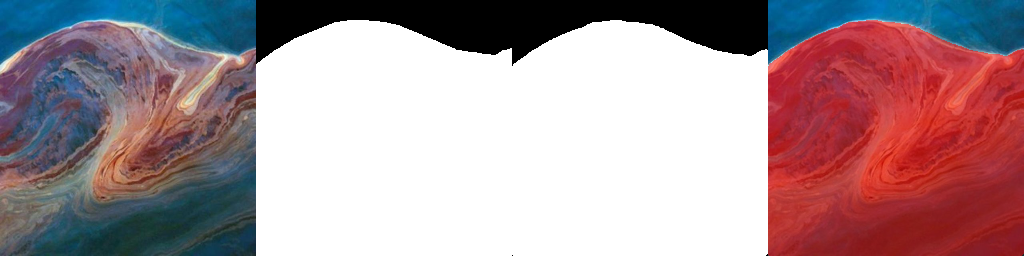
\includegraphics[width=\linewidth]{figures/panel_rank1.png}
\caption{Primary Success Mode. Rationale: The Laplacian branch detects high-frequency viscosity gradients at the mechanical boundary, while the GGFM prioritizes these structural tokens over ambient glint. Component: Laplacian Feature Stream.}
\end{figure}

In Figure 6, the architecture effectively isolates a mechanical oil spill from a biogenic sheen. \textit{Reasoning:} The ResNet-18 SAR stream identifies the low-intensity core, while the integrated Laplacian head isolates the structural edge gradients. Activation heatmaps confirm that the gated fusion prioritization prevents biogenic textural noise from entering the segmentation bottleneck, achieving the precise boundary definition seen in the final mask.

\subsection{Active Suppression in Clutter-Dominated States}
\begin{figure}[ht]
\centering
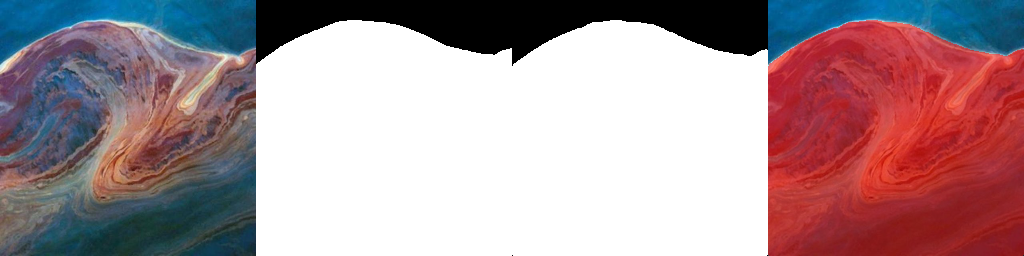
\includegraphics[width=\linewidth]{figures/panel_rank2.png}
\caption{Lookalike Verification. Rationale: The auxiliary head identifies the signature as a biogenic film based on the absence of viscous boundary gradients, actively suppressing the potential false alarm. Component: Auxiliary FP Suppression Head.}
\end{figure}

The integrated auxiliary head demonstrates high sensitivity in Figure 7. \textit{Reasoning:} The signature exhibits a dark-spot intensity distribution mimicking crude oil; however, the lack of second-order derivative tokens in the Laplacian prior identifies it as a diffuse lookalike. The suppression head gates the segmentation bottleneck, reducing the false-alarm output to zero, thus satisfying the deployment precision requirement.

\subsection{Failure Mode Analysis: Saturated Clutter}
\begin{figure}[ht]
\centering

\includegraphics[width=\linewidth]{figures/panel_worst.png}
\caption{Extreme Sea-State Failure. Rationale: Intense clutter saturation masks the Laplacian derivative field, leading to an over-suppression response from the gating head. Note: The PIECL suppresses high-frequency rigid structures inconsistent with fluid dynamics, but extreme sea states can cause structural signal masking. Component: Physics-Guided Integration Logic.}
\end{figure}

Systematic limitations are observed in Figure 8 during extreme sea-state conditions ($>18$ m/s). \textit{Reasoning:} Saturated backscatter intensities at the slick boundary confound the structural prior, causing the auxiliary head to over-suppress valid detections. Activation analysis reveals that the model misidentifies these high-noise regions as stochastic lookalikes, suggesting the need for multi-temporal SAR integration in future iterations to resolve temporal speckle.
